\documentclass[journal abbreviation, manuscript]{copernicus}
\usepackage{comment} 

\begin{document}

 %% \ SECTION 3
\section{Use cases}

\begin{comment}
Andrew Comments:

Structure: just go through it, Use Case I, Use Case II, Use Case II. No Methods & Results section

go through it from front to back, explain what an NPZD model is.
"We recreate the NPZD model formulation by Anderson, in the model there is one .." describe equations in words. Then say See Anderson et al. or appendix X for full equations

My Comments:
Notes from Banas, 2011 (reading it now):
- "NPZ-model" 
- "mechanistically simple"
- "resolves one level of trophic interaction in detail"
- he says dis thing goes stable in a cycle after 10 - 20 years?! well it is the NPZ, without light, etc. so makes sense
- should i do a chemostat instead? this could be the slight modification, that makes sense to include

keep in mind, this would mean, that I have both a slightly different version of EMPOWER
and a slightly different version of ASTroCAT
but still a very similar version of example 3.

This will make the whole story come together nicely!
\end{comment}

% PARAGRAPH STARTS HERE:
To showcase the utility of the phydra package for modelling marine ecosystems, we demonstrate three model implementations of varying complexity.

The phydra package was designed specifically to allow for the implementation of flexible dimensionality, as described in Section 2. For the following use cases we focus on varying food web complexity in relatively simple zero-dimensional physical settings. 

All presented models could be run in one, two or three-dimensional physical schemes, by providing the appropriate setup grid and processes defining physical interactions between grid points. Our choice of zero-dimensional implementations was motivated by the fact that such physical schemes are much easier to set up and analyse.  The online documentation of the phydra package provides simple examples of multi-dimensional marine ecosystem models.

All model structures present highly idealised versions of marine plankton assemblages. Use case 1 is a canonical NPZD ecosystem model embedded in slab physics. The specific implementation is adapted from Anderson et al. 2015. 

The second use case is an example of a more complex size-structured food web, implemented in the minimalistic physical setting of a flow-through system. This specific implementation is adapted from Banas, 2011.



% in final version, present: - jupyter notebook for each example, add links in text

\subsection{Forcing and verification data}

some text here on forcing and verification, where it's from, how it's done


\subsection{Use case 1: NPZD slab model}
%  quickly explain overview, explain methods for all of them shortly, with schematics, and put full system of equations & parameter tables in the Appendix!

Use case 1 is a canonical NPZD ecosystem model embedded in slab physics. The ecosystem is embedded in an upper mixed layer that is affected by variable mixing with an inert deeper layer driven by the mixed layer depth (MLD) forcing. The model contains only four state variables, namely a nutrient  (nitrate), phytoplankton, zooplankton and detritus, but has more complicated treatments of light-limitation and water column dynamics. The specific implementation is adapted from the elegant EMPOWER model by Anderson et al. 2015. 

One benefit of the implementation in phydra is the added flexibility and speed, that object-oriented code offers over procedural scripts and hard-coded for loops as time steps containing the model calculations. (I should only say this if my model is faster than EMPOWER). The package is particularly well suited for model testing and prototyping in the interactive jupyter notebook environments. 

\subsusection{Model Structure: NPZD}
explain model structure in words, reference equations in appendix

\subsubsection{Physical setting: slab}
explain slab physics, equations in appendix



\subsubsection{NPZD slab model results}
show and explain results, as simple as possible, full parameters/sensitivity analysis in appendix?


\subsection{Use Case 2: Size-structured chemostat model}

This specific system could be described as a chemostat, where constant nutrient addition drives the growth of multiple state variables of phytoplankton and zooplankton. Each plankton state variable is assigned a size measured as the equivalent spherical diameter (ESD). The ESD determines the nutrient uptake parameters, growth rates and grazing susceptibility via size-based allometries taken from meta-analysis of laboratory data.

\subsection{Model Structure: size-structured NPZ}

\subsubsection{Physical setting: chemostat}


\subsubsection{Model results}


\subsection{Use Case 2: Size-structured chemostat model}

\subsection{Model Structure: size-structured NPZD}



\subsubsection{Physical setting: slab}

\subsubsection{Model results}


\clearpage
% Figures

%%f
\begin{figure*}[t]
\includegraphics[width=15cm]{Figures/firstdraft_plots/01_forcing_labeled.pdf}
\caption{(a) Map shows locations of the two comparative model runs. Each square is of side length 4° centered on 47°N ,-20°E and 0°N,-20°E respectively. Environmental forcings are averaged across area. (b) Forcing is shown: Mixed Layer Depth (MLD), Nitrate below the Mixed Layer (N0),
Photosynthetically Active Radiation (PAR) and temperature averaged across the Mixed Layer (TMLD)}
\label{phydraforcing}
\end{figure*}



%%f
\begin{figure*}[t]
\includegraphics[width=15cm]{Figures/firstdraft_schematics/02__schematics_NPZDandChemostat.pdf}
\caption{TEXT}
\label{phydraschematics_1}
\end{figure*}


%%f
\begin{figure}[t]
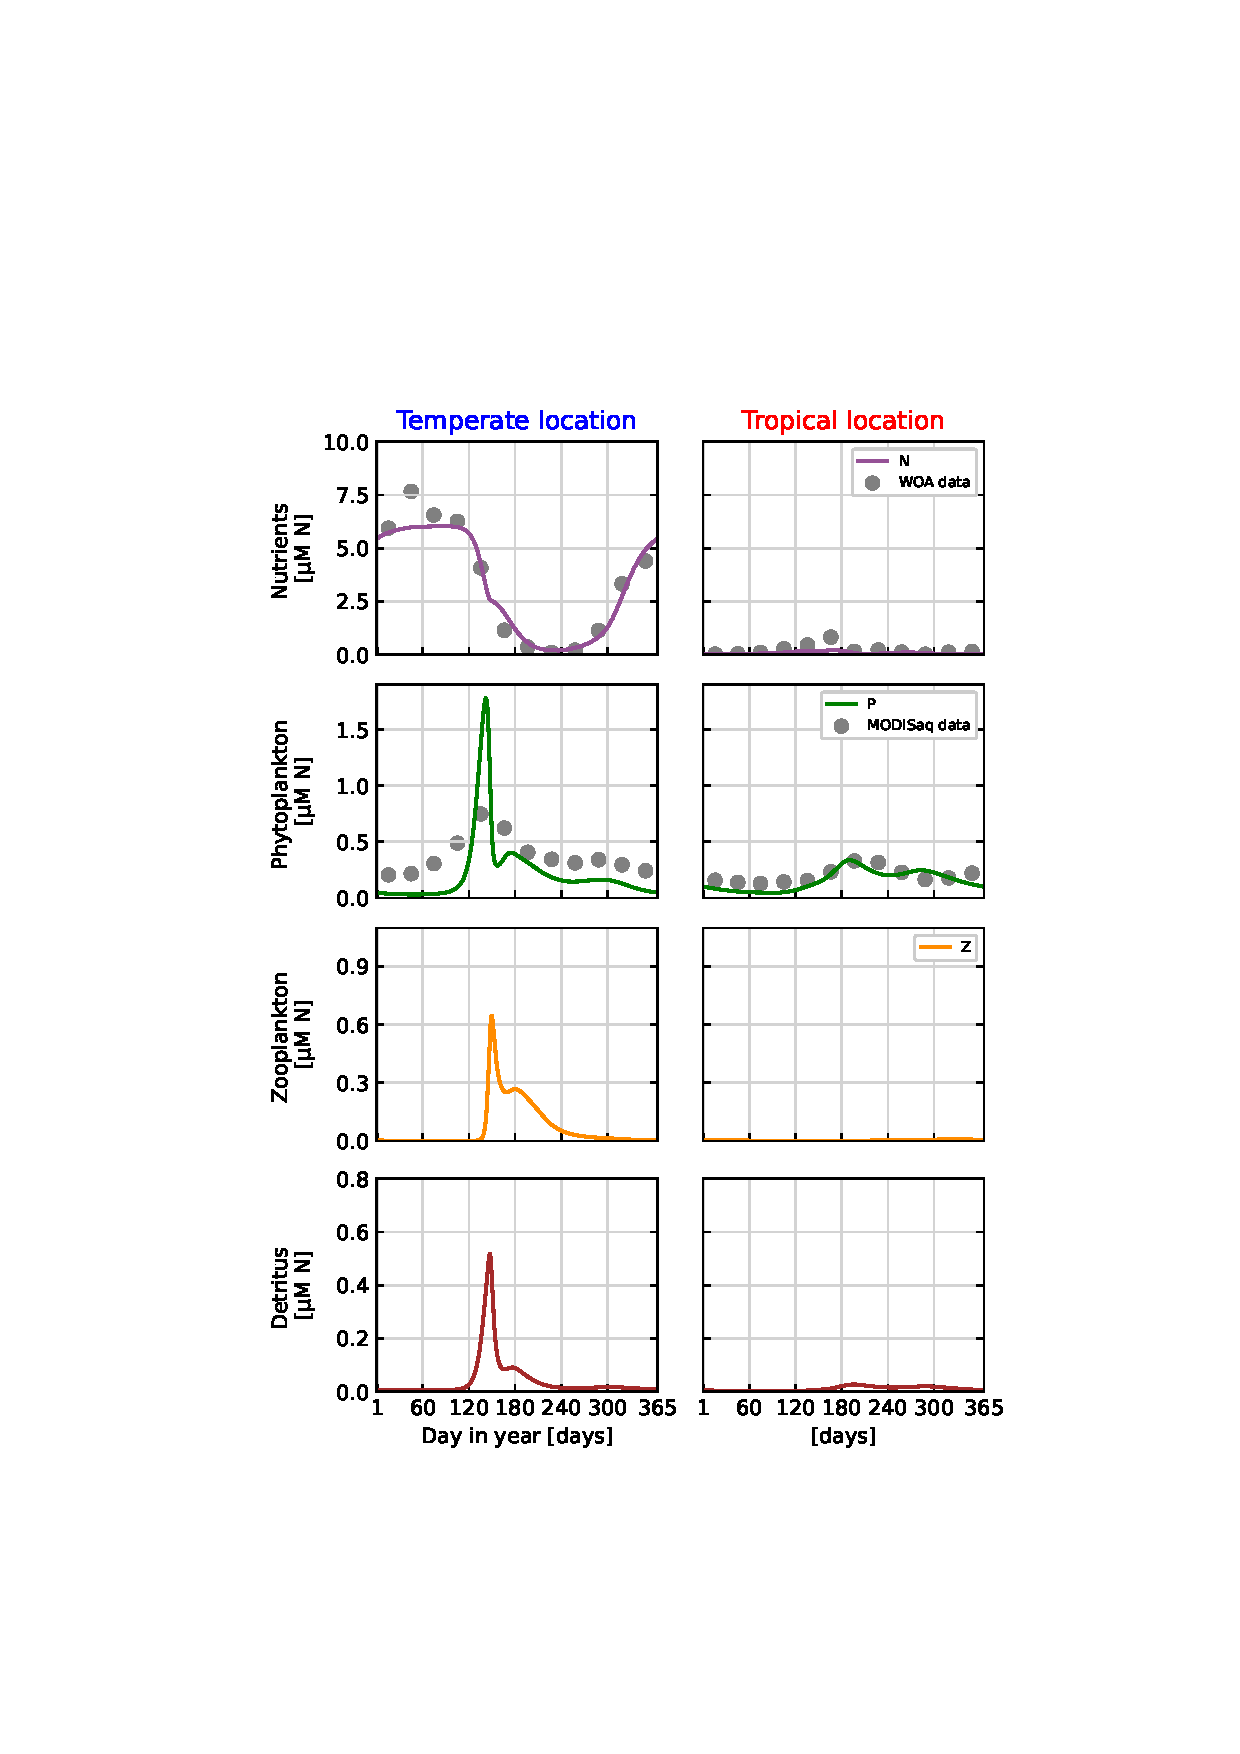
\includegraphics[width=6cm]{Figures/firstdraft_plots/02_NPZDslab.pdf}
\caption{TEXT}
\end{figure}

%%f
\begin{figure}[t]
\includegraphics[width=6cm]{Figures/firstdraft_plots/03_chemostat.pdf}
\caption{TEXT}
\label{ASTroCAT_plot}
\end{figure}

%%f
\begin{figure*}[t]
\includegraphics[width=10cm]{Figures/firstdraft_schematics/03__schematics_SizeStructSlab.pdf}
\caption{TEXT}
\label{phydraschematics_3}
\end{figure*}



%%f
\begin{figure*}[t]
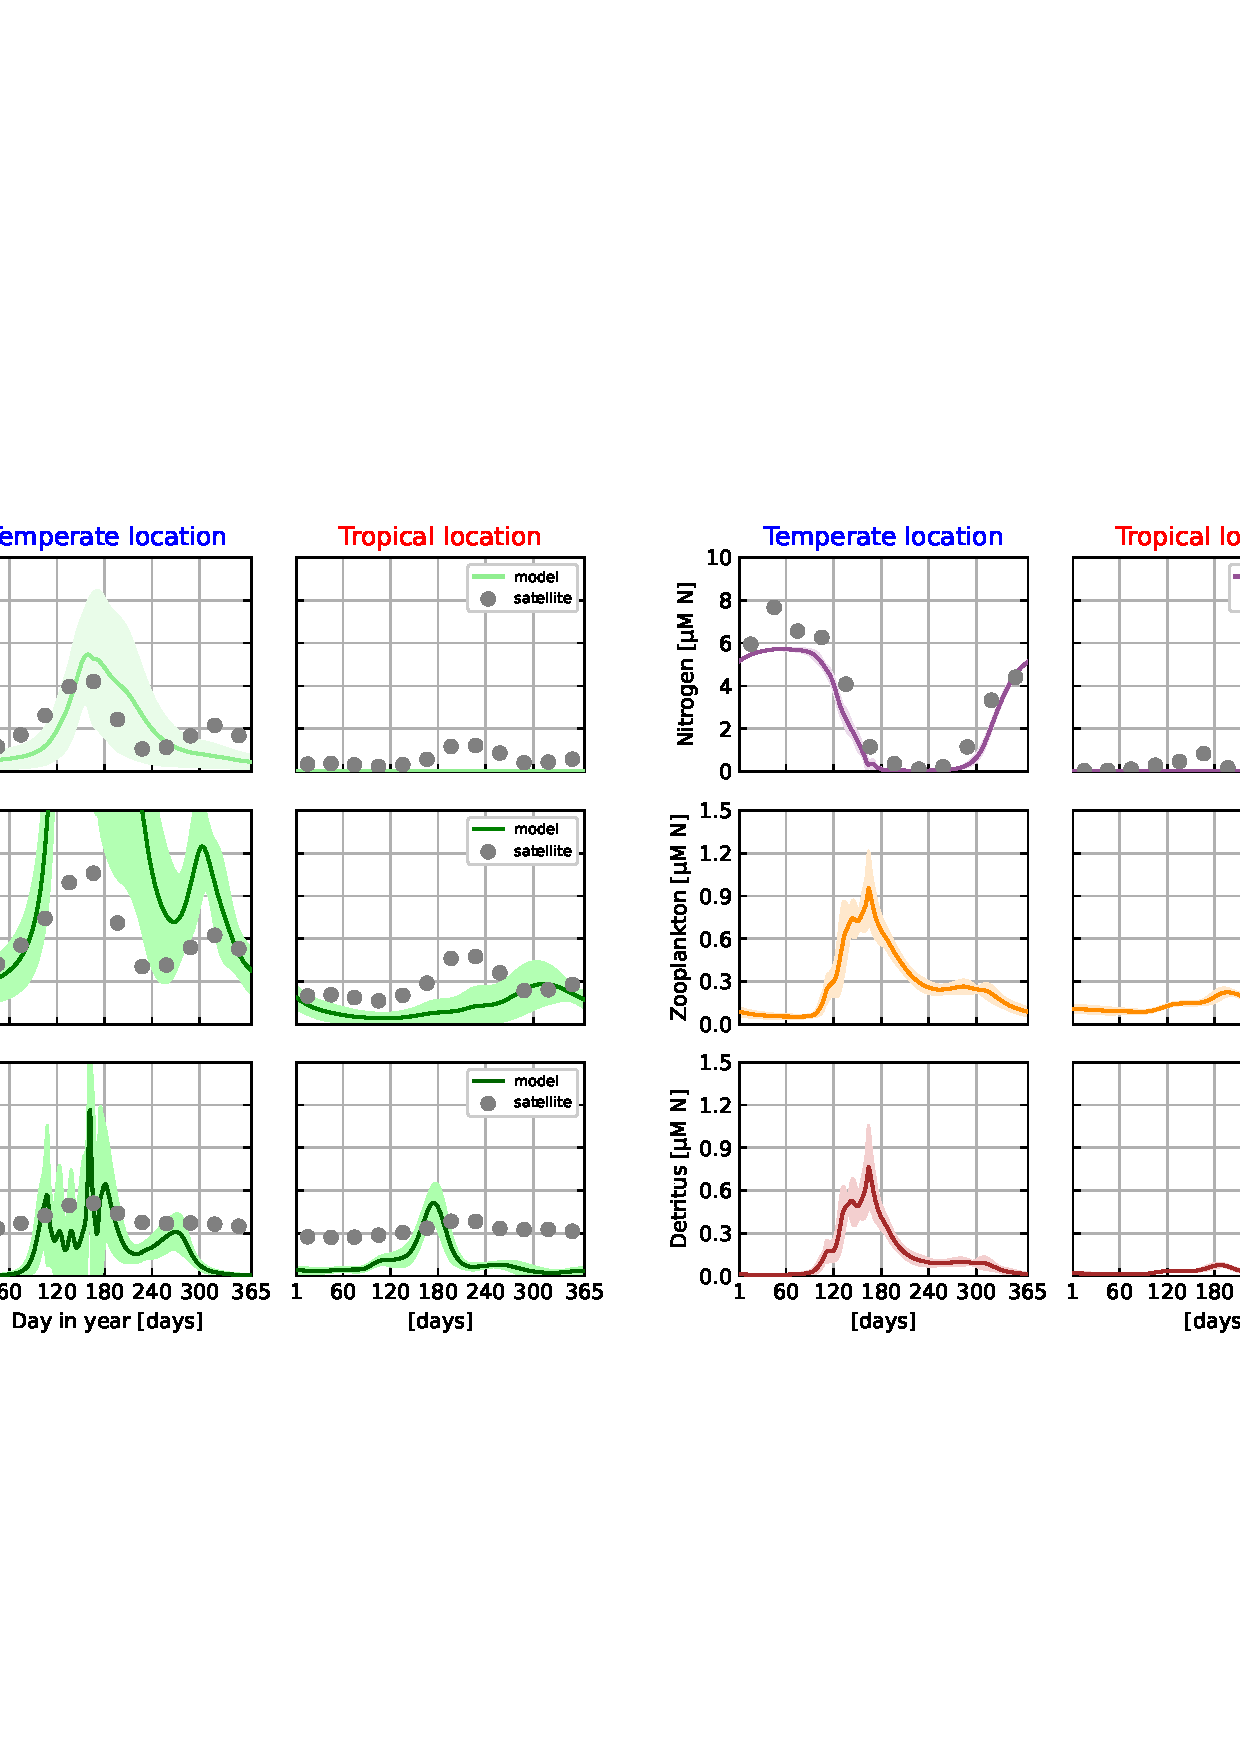
\includegraphics[width=12cm]{Figures/firstdraft_plots/04_sizestruct_slab.pdf}
\caption{TEXT}
\label{ASTroCAT_plot}
\end{figure*}
% Tables

\end{document}